\subsection{Keypoint-Based Visual SLAM}
\label{sec:kv_slam_background}

SLAM is the joint problem of simultaneously generating a map of an environment and estimating the position of an observer within that map based on sensor observations. First explored in the 1980s \cite{smithEstimatingUncertainSpatial1988}, SLAM has become a de facto standard in robotics for tasks which require operations within unfamiliar environments. A wide variety of sensors can be utilized by SLAM, the most common being LiDAR, cameras, and RGBD sensors. The high level relationships between these sensor modalities are shown in Figure \ref{fig:slam_family_tree}. Keypoint-Based Visual SLAM refers to a subset of the wider SLAM ecosystem characterized by the use of cameras as the primary sensor, and image features extracted from images as the primary data for tracking and mapping.

\begin{figure}[!ht]
    \centering
    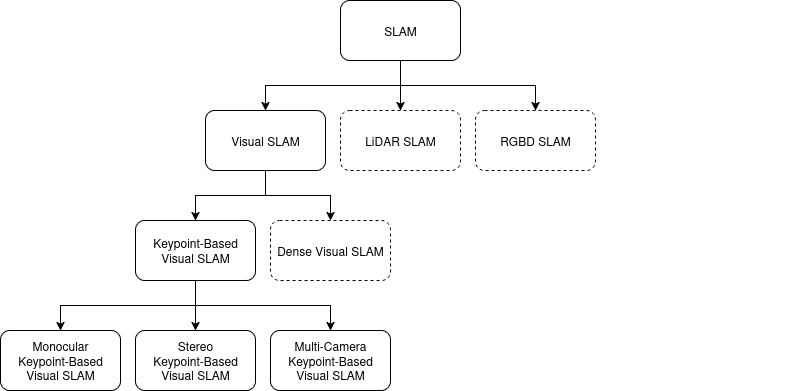
\includegraphics[width=0.9\textwidth]{resources/slam_family_tree.png}
    \caption[SLAM Family Tree]{Overview of the relationships between popular SLAM modalities.}
    \label{fig:slam_family_tree}
\end{figure}

The first implementations of KV-SLAM came in the early 2000s \cite{seMobileRobotLocalization2002}\cite{davisonRealtimeSimultaneousLocalisation2003}, making the field relatively young. This can be attributed to the difficulty in estimating 3D geometries from 2D images, unlike LiDAR and RGBD which are capable of direct 3D environmental measurements. However, due to the extremely low cost and wide availability of camera sensors, KV-SLAM is a popular modality for robotics, AR/VR, and autonomous driving applications.

An overview of KV-SLAM concepts is provided below, followed by a discussion of the KV-SLAM subsystems which are relevant to this research. The internal operations of KV-SLAM are highly dependent on implementation details, so explanations will relate to the ORB-SLAM3 KV-SLAM implementation. ORB-SLAM3 is a popular open source implementation of KV-SLAM which is widely used in research due to its performance, open-source codebase, and usage of methods and techniques that are well-documented and widely accepted.